\documentclass[10pt,a4paper]{article}
\usepackage[utf8]{inputenc}
\usepackage[portuges]{babel}
\usepackage{a4wide}
\usepackage{indentfirst}
\usepackage{graphicx}
\usepackage{color}
\usepackage[dvipsnames]{xcolor}
\begin{document}

\begin{titlepage}
\center 
\newcommand{\HRule}
{\rule{\linewidth}{0.4mm}}
\textsc{\LARGE Universidade do Minho}\\[0.4cm]
\vspace{1cm}
\textsc{\large Mestrado Integrado em Engenharia Informática}\\[1.5cm]

\includegraphics[scale=1.2]
{UM}\\[0.5cm]
\vspace{0.5cm}
\HRule \\[1cm]
{\Huge \bfseries Projeto de Laboratórios de Informática III} \\[0.7cm]
\HRule \\[1cm]
\vspace{0.1cm}
\textsc{\Large \textbf{Grupo 41}}\\[0.75cm]
\vspace{0.1cm}
{\large{Ana Ribeiro(A82474) \qquad Jessica Lemos(A82061) \qquad Pedro Pinto (A82535)}}\\[0.8cm]
\vspace{7cm}
{\large\today}\\[2cm] 
\vfill 
\end{titlepage}

\thispagestyle{empty}
\cleardoublepage

\thispagestyle{empty}
\tableofcontents
\cleardoublepage
\pagenumbering{arabic}
\setcounter {page}{1}

\section{Introdução}

Este relatório aborda a elaboração do mesmo projeto realizado na primeira fase da disciplina de Laboratórios de Informática 3 (LI3), do Mestrado Integrado em Engenharia Informática da Universidade do Minho, na linguagem de programação Java. 
Este projeto consiste na implementação de um sistema capaz de processar ficheiros XML que armazenam as várias informações utilizadas pelo Stack Overflow. Uma vez processada essa informação, pretende-se que seja possivel executar um conjunto de interrogações específicas, apresentadas posteriormente, de forma eficiente.

\cleardoublepage

\cleardoublepage

\section{Concepção}
\label{sec:solucao}

\subsection{Concepção do problema}

Tendo em conta o problema apresentado, decidimos organizar o nosso trabalho em dois grupos:

\begin{itemize}
 \item Posts
 \item Users
\end{itemize}

Para realizar as queries relativas aos posts é necessário obter do ficheiro \textit{"Posts.xml"} as seguintes informações: o id e o tipo do post e no caso de este ser uma resposta guardar o id da respetiva pergunta, as tags, o seu título, o id do utilizador que o elaborou, a sua data de criação e o número de comentários. Caso o post seja uma pergunta terá de se guardar também o número de respostas. A fim de tornar a resolução das interrogações deste grupo eficientes, é evidente a necessidade de implementar uma estrutura onde seja rápida a procura dos posts de uma dada data. Acrescido a esta preocupação, é indispensável ter o cuidado de organizar os posts de uma data pelo seu id.\\
 \indent  Quanto aos users, é oportuno guardar do ficheiro \textit{"Users.xml"} o id, o nome, a reputação e a informação do seu perfil. Para tornar eficaz a resolução destas queries, é útil estruturar as informações pelo seu id.\\
 \indent Para as tags, é preciso armazenar do ficheiro \textit{"Tags.xml"} o id e o seu nome, ordenadas por este.

\subsection{Concepção da solução}
 Com o objetivo de solucionar todas as interrogações do grupo dos posts de modo eficiente utilizamos uma \textit{HashMap} organizada por datas, em que cada posição contém uma \textit{TreeMap} com todos os posts dessa data ordenada pelo seu id. A escolha da \textit{HashMap} deveu-se ao elevado número de interrogações que envolviam intervalos de tempo, para estas tornou-se imperativo evitar percorrer os posts que não tivessem incluídos nesse intervalo. Uma vez reduzida a procura, foi necessário organizar a \textit{TreeMap} pelo o id do post, dado que a maioria das interrogações se baseiam neste fator.\\
 \indent Para os users optamos por uma \textit{HashMap} organizada pelos ids dos utilizadores, dado que todas as queries deste grupo se baseiam no id. Houve também a necessidade de associar a cada user um \textit{ArrayList} com todos os posts em que participou.\\
 \indent Tendo em conta que para o grupo das tags a procura se baseia no seu nome definimos uma \textit{HashMap} disposta por este. \\
\indent Para auxiliar estes dois grupos foi fundamental recorrer a dois \textit{ArrayLists} para diminuir o tempo de resolução de interregações que envolviam tops. Um destes incluía os utilizadores estruturados pela sua reputação e o outro engloba os utilizadores ordenados pelo número de posts realizados.
\cleardoublepage
\section{Classes}
\label{sec:solucao}
Nesta secção iremos abordar a estrutura do nosso projeto, referindo as classes presentes, os
atribuitos e o modo de funcionamento de cada uma.

\subsection{Parse}
Para resolver as queries propostas é necessário realizar o \textit{parsing} que consiste em percorrer cada um dos ficheiros e armazenar na estrutura a informação que consideramos relevante.
Desta forma, para fazer o parse dos ficheiros \textit{xml} recorremos à \textit{API} do \textit{Stax}. 
Numa fase inicial, testamos elaborar o parse utilizando a \textit{API} do \textit{DOM}. No entanto, este não era o método mais adequado, uma vez que carrega toda a informação para a memória.

\subsection{Struct}
Esta classe é fundamental no nosso trabalho, dado que armazena a informação de todos os users, posts e tags. A estrutura principal utilizada inclui três \textit{Maps} relativos aos users, posts e tags, e ainda dois \textit{Lists} úteis nas resolução de determinadas interrogações. É importante salientar que o \textit{Map} da estrutura dos posts inclui em cada posição um \textit{Map} com os posts dessa data. Quanto aos users cada posição da \textit{Map} encontra-se associada a uma \textit{List} com os posts realizados por este. 

A escolha dos \textit{Maps} deve-se à simples implementação e eficiente procura. Como não será necessário aceder a nenhuma posição diretamente decidimos optar por um \textit{List}. Esta opção deveu-se também à fácil ordenação dos valores.

\begin{center}
\graphicspath{ {/home/jessica/Desktop/} }
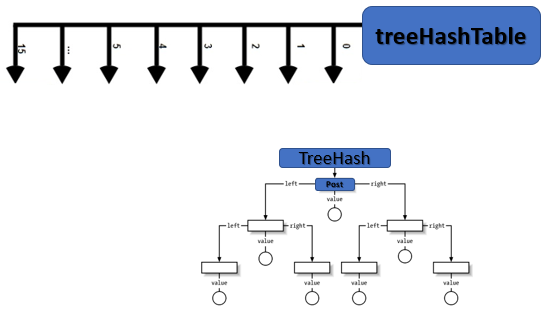
\includegraphics[width=7cm]{Posts}
\end{center}

Na imagem acima encontra-se representada a estrutura dos posts constituída por uma \textit{HashMap} em que cada posição contém uma \textit{TreeMap} com os \textit{Posts} realizados nesse dia.

\begin{center}
\graphicspath{ {/home/jessica/Desktop/} }
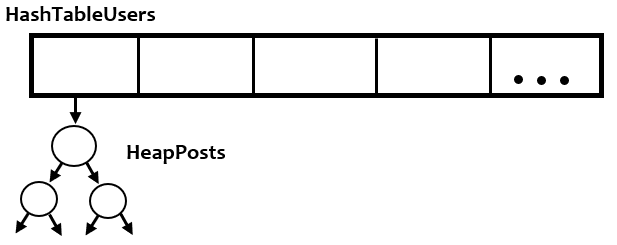
\includegraphics[width=8cm]{Users}\\
\end{center}

Nesta, encontra-se esquematizado a estrutura dos users composta por uma \textit{HashMap} com os utilizadores que têm associado um \textit{ArrayList} com alguma informação de todos os seus posts.

\begin{center}
\graphicspath{ {/home/jessica/Desktop/} }
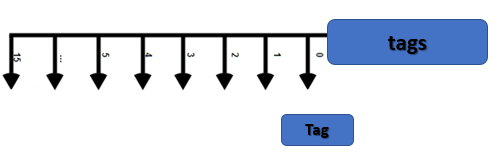
\includegraphics[width=6cm]{Tags}\\
\end{center}

Por último, podemos visualizar a estrutura das tags que corresponde a uma \textit{HashMap} com as tags ordenadas pelo seu nome.

\subsection{TreeHash}
Esta classe contém a data de criação dos posts que se encontram armazenados numa \textit{TreeMap}, bem como dois contadores, um com o número de posts tipo resposta e outro com o número de posts tipo pergunta, que serão úteis para a realização de determinadas queries.

\subsubsection{Post}

Esta inclui todas as informações relativa aos posts, nomeadamente:
\begin{itemize}
\item id - id do post
\item postTypeId - tipo do post
\item parentId - id da pergunta correspondente
\item tag - tags do post
\item title - título do post
\item ownerUserId - id do criador do post
\item answerCount - número de respostas ao post
\item commentCount - número de comentários ao post
\item score - pontuação do post
\end{itemize}

\subsection{Users}
Esta classe contém as informações dos users bem como um \textit{ArrayList} com os posts de cada um, para a resolução de duas das interrogações: \textit{getUserInfo} e \textit{bothParticipated}, e ainda uma variável que conta o número total de posts realizados pelo utilizador.\\

\indent Deste modo, a classe é constituída por:
\begin{itemize}
\item ownerUserId - id do utilizador
\item displayName - nome do utilizador
\item reputation - reputação do utilizador
\item nPosts - número de posts realizados pelo utilizador
\item aboutMe - short bio do utilizador
\item userList - posts do utilizador (id e data de criação do post)
\end{itemize}

\subsection{Tag}

Esta é composta pelas seguintes informação retirada do ficheiro \textit{Tags.xml}:
\begin{itemize}
\item id - id da tag
\item tagName - nome da tag
\end{itemize}

\subsection{maxMap}
Foi imperativo a criação desta classe para a realização da query \textit{mostAnsweredQuestions} para poder ordenar de acordo com o requerido como será explicado na secção das \textit{Queries}. Para tal precisamos das seguintes informações:
\begin{itemize}
\item id - id do post
\item count - fator de ordenação
\item flag - indica se determinada condição se verifica
\end{itemize}

\subsection{maxList}
Esta classe foi útil para ordenar os posts de acordo com a data de criação destes. Sendo assim constituída por:
\begin{itemize}
\item id - id do post
\item creationDate - data de criação do post
\end{itemize}

\subsection{maxPosts}
Classe utilizada para ordenar os posts ou utilizadores de acordo com um contador, que varia consoante a situação. Contendo a seguinte informação:
\begin{itemize}
\item id - id do post ou do utilizador
\item nPosts - contador
\end{itemize}

\subsection{Comparators}
Tendo em conta a necessidade de ordenação dos posts e dos users tornou-se imperativo a criação de comparators que indica à estrutura a forma como ordenar a informação.
Desta forma, foram criados três comparators:
\begin{itemize}
\item maxMapComparator - ordena a informação da classe \textit{maxMap} de acordo com o contador
\item DataComparator - ordena a informação de acordo com a data
\item maxPostsComparator - ordena a informação da classe \textit{maxPosts} de acordo com o contador
\end{itemize}

\subsection{Queries}
\subsubsection{Load}
Esta interrogação é a mais demorada visto que é responsável por processar a informação dos ficheiros e armazená-la na nossa estrutura. Nesta também procedemos à inicialização da estrutura.

\subsubsection{Info\_from\_post}
Começamos por procurar o post na \textit{treeHashTable} e caso este seja do tipo pergunta retiramos-lhe o título e id do utilizador. Com o id acedemos à estrutura dos users e obtemos o nome do utilizador. Na eventualidade do post ser do tipo resposta retiramos o id da pergunta a que corresponde e efetuamos o proceso anterior para este.

\subsubsection{Top\_most\_active}
Recorrendo ao \textit{ArrayList topN} que se encontra ordenado pelo número de posts de cada utilizador, extraimos os N ids pedidos e criamos a lista necessária para devolver. 

\subsubsection{Total\_posts}
Para esta query percorremos a \textit{treeHashTable} e no caso de a data pertencer ao intervalo de tempo pertendido, somamos aos contadores do número de respostas e número de perguntas respetivamente, e de seguida criamos o par esperado com essa informação.

\subsubsection{Questions\_with\_tag}
Iniciamos por percorrer a \textit{treeHashTable} e na hipótese de a data estar contida no intervalo de tempo desejado, vamos a todos os posts e na eventualidade de um ser do tipo pergunta, verificamos se a tag dada se encontra nas tags do post. Em caso afirmativo, guardamos num \textit{ArrayList} o id e a data do post (maxList) para posteriormente ordená-la de acordo com a data e de seguida criamos a lista com os ids dos posts a devolver.

\subsubsection{Get\_user\_info}
Nesta interrogação acedemos à posição onde se encontra o utilizador pretendido na \textit{userHashTable} e obtemos a informação do seu perfil e retiramos o \textit{ArrayList} integrante, que posteriormente é ordenado de modo a obter os seus dez últimos posts.

\subsubsection{Most\_voted\_answers}
Começamos por percorrer a \textit{treeHashTable} e na possibilidade de a data se enquadar no intervalo de tempo pedido, acedemos a todos os posts e caso seja do tipo resposta inserimos o score e o id no \textit{ArrayList} constituído por maxPosts de modo a ordenar e retirar o top N pretendido.

\subsubsection{Most\_answered\_questions}
Nesta interrogação tornou-se imperativo a criação de uma \textit{HashMap constituído por maxMaps}.
Para esta query passamos por todas as posições da \textit{treeHashTable} e no caso da data se encontrar no intervalo requerido percorremos os posts verificando se são do tipo pergunta ou resposta. Na eventualidade de ser do tipo pergunta, colocamos a flag a 1 na \textit{Map} indicando que a pergunta se encontra no intervalo pretendido, caso contrário aumentamos ao count (número de respostas ao post). No final, copiamos para uma lista as maxMaps com flag a 1 para posteriormente ordená-las e obter os N pretendidos.

\subsubsection{Contains\_word} 
Passamos por todos os Posts existentes e na eventualidade de ser do tipo pergunta verificamos se a palavra dada se encontra no título. Em caso afirmativo, inserimos a \textit{maxList} com o id e a data do post no \textit{ArrayList} de modo a no fim ordenarmos e retirar o top N pretendido.

\subsubsection{Both\_participated} 
Começamos por aceder às posições da \textit{userHashTable} dos utilizadores solicitados e retiramos os respetivos \textit{ArrayLists}. Inserimos os ids do maior \textit{ArrayList} noutro \textit{ArrayList}, mas caso o post a inserir seja do tipo resposta, guardamos o id da pergunta correspondente. De seguida, percorremos os elementos do outro \textit{ArrayList} e verificamos se é do tipo pergunta ou tipo resposta. Na eventualidade de ser do tipo pergunta, verificamos se o id deste se encontra no \textit{ArrayList} criado anteriormente. Caso contrário, retiramos o parentId e utilizamos este como fator de comparação.

\subsubsection{Better\_answer} 
Nesta query, percorremos a \textit{treeHashTable} e os posts da  \textit{TreeHash} até encontrar o post requerido e retiramos o número de respostas existente. Depois voltamos a percorrer a \textit{TreeHashData} e sempre que encontramos um resposta ao post vamos buscar as informações necessárias para obter a média ponderada e decrementamos ao número de respostas existentes, pois deste modo evitamos continuar a percorrer a estrutura quando já não houverem mais respostas à pergunta. Sempre que encontramos uma média maior do que a guardada até ao momento, substituimos esse valor e atualizamos o id.

\subsubsection{Most\_used\_rep} 
Iniciamos por preencher um \textit{ArrayList} com os ids dos N utilizadores com melhor reputação. De seguida percorremos a \textit{treeHashTable} e se a data da posição pertencer ao intervalo de tempo, acedemos aos posts da \textit{TreeHash} e para cada um verificamos se o utilizador está incluido no top N estabelecido anteriormente. Caso tal se suceda, para todas as tags desse post vamos verificar se o seu id já se encontra na \textit{HashMap} constituída por \textit{MaxPosts} e caso esteja incrementamos o número de vezes que esta ocorre. Caso contrário, vamos procurá-la à estrutura das tags e inserimos o seu id na nossa \textit{HashMap}. Posteriormente os elementos da \textit{HashMap} são inseridos num \textit{ArrayList} de modo a obtermos as N tags mais usadas pelos N utilizadores com melhor reputação.\\

\subsubsection{Clear} 
Percorremos todas as estruturas criadas libertando as informações para o qual foi alocada memória.
\cleardoublepage
\section{Conclusão}
Assim como na primeira fase do projeto, também nesta a escolha das estruturas tiveram influência direta no desempenho das interrogações requeridas. No entanto, a utilização da linguagem Java tornou este resolução muito mais simples uma vez que não tivemos de criar tabelas de hash ou árvores binárias pois o Java contém muitas estruturas pré definidas eficientes.\\
\indent Na realização desta fase tentamos corrigir as falhas apontadas na fase anterior. Assim, alteramos algumas das nossas estruturas com o objetivo de reduzir o nosso tempo de load sem comprometer significativamente o tempo de resolução das queries. Apesar de este objetivo ter sido atingido consideramos que ainda existem alguns aspetos a melhorar neste projeto.\\
\indent Em última instância, consideramos que os nossos objetivos neste projeto foram alcançados.
\end{document}